\begin{figure}[!htbp]
    \centering
    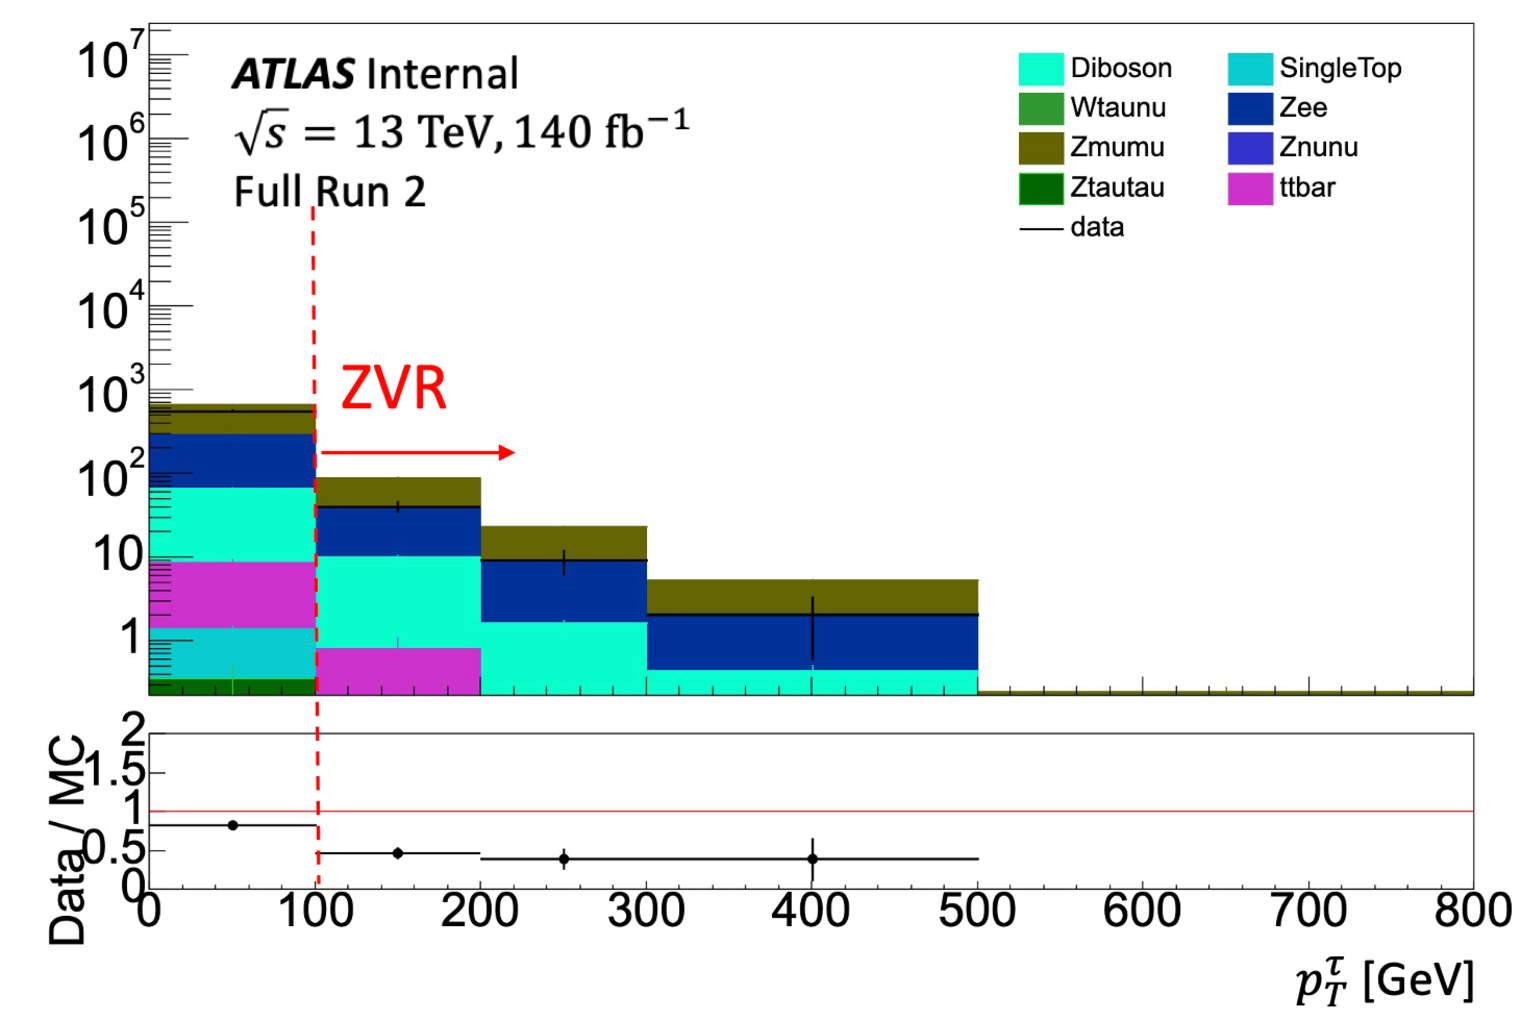
\includegraphics[width=0.80\linewidth]{Figs/CH8/ZVR_pTtau.pdf}
    \caption[Pre-fit tau momentum distribution in the ZVR]{Pre-fit $N-1$ distribution of $\pT^\tau$ in the ZVR. The red arrow indicates the $100~\GeV$ threshold. The lower panel compares data with the total simulation. The high-$\pT^\tau$ prediction exceeds the observed yield.}
    \label{fig:ch8_zvr_pt}
\end{figure}

\begin{figure}[!htbp]
    \centering
    \begin{subfigure}{0.47\linewidth}
        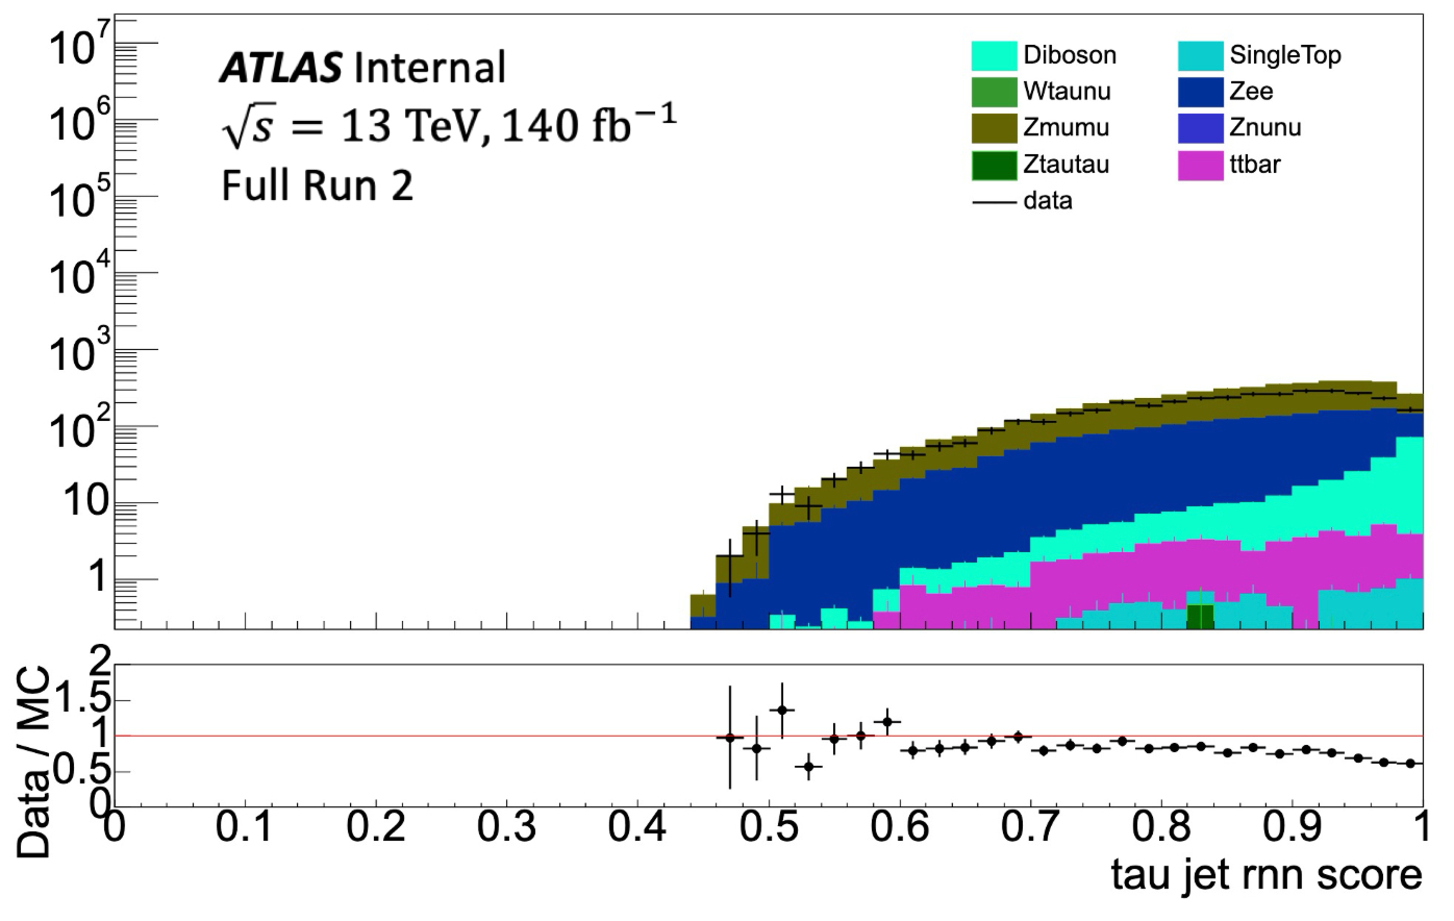
\includegraphics[width=\linewidth]{Figs/CH8/ZVR_1tau20GeV_score.pdf}
        \caption[]{$\pT^\tau>20~\GeV$}
    \end{subfigure}\hfill
    \begin{subfigure}{0.47\linewidth}
        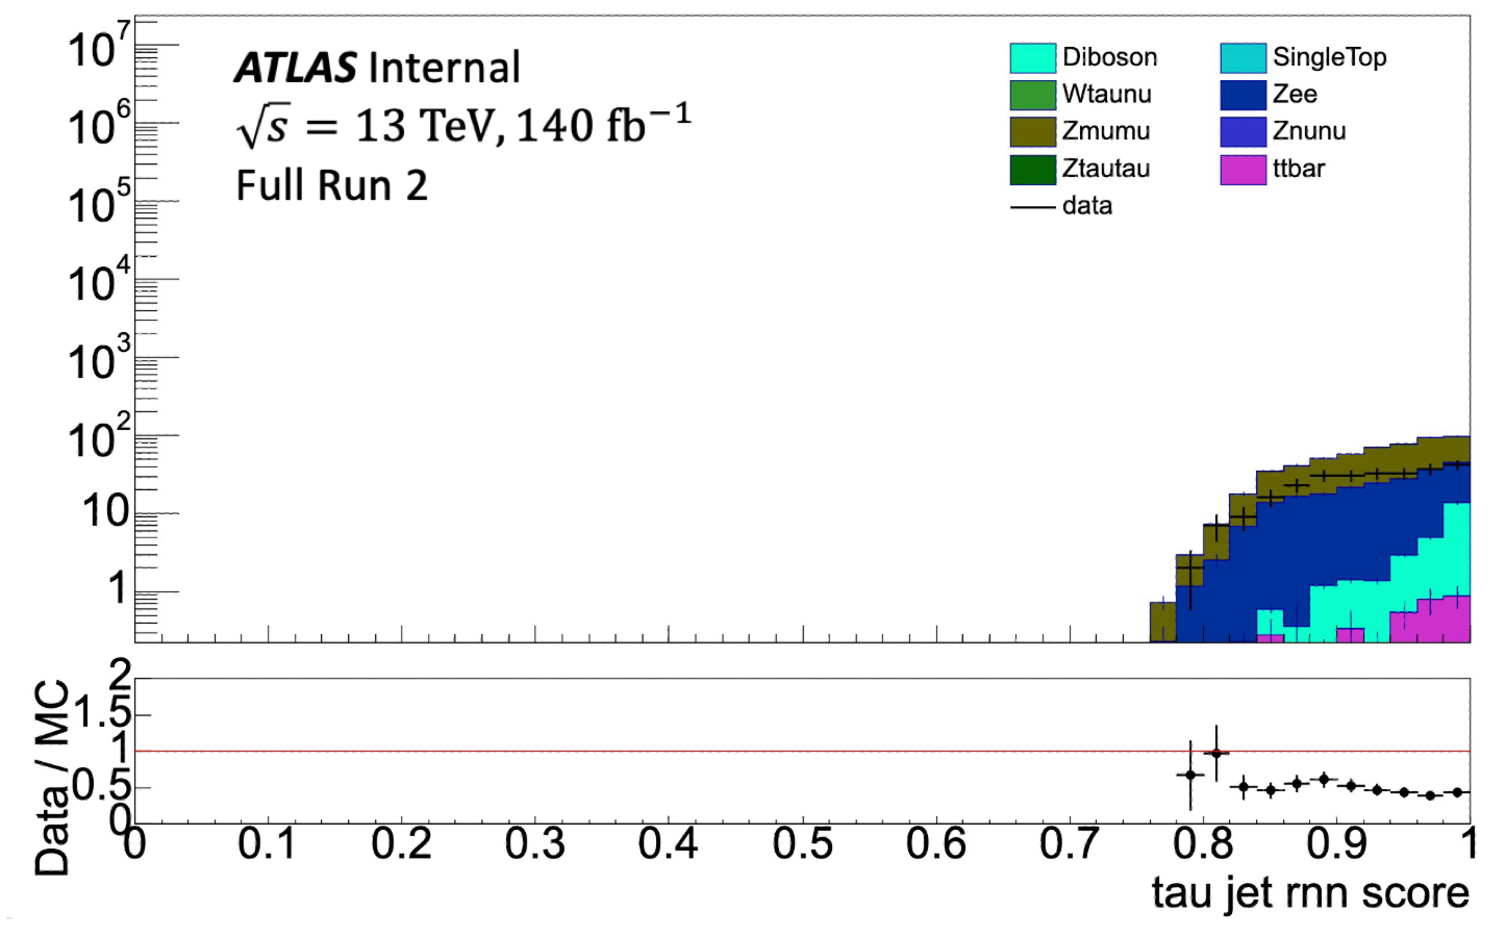
\includegraphics[width=\linewidth]{Figs/CH8/ZVR_1tau100GeV_score.pdf}
        \caption[]{$\pT^\tau>100~\GeV$}
    \end{subfigure}\par\medskip
    \caption[Tau-identification RNN distributions in the ZVR]{The $\tau$-identification RNN score in $Z$+jets-enriched samples with (a) $\pT^\tau>20~\GeV$ and (b) $\pT^\tau>100~\GeV$. Looser $\tau$ identification and a relaxed transverse-mass requirement are used to compare the low- and high-score regions. These selections differ from the nominal ZVR.}
    \label{fig:ch8_zvr_rnn}
\end{figure}
